\chapter{数据集数据库系统安全}
\question{什么是数据库}
按照数据结构来组织、存储和管理数据的仓库。

\question{数据备份}
将数据已某种方式保留,当系统遭到破坏或者其他特定情况下重新加以利用。其核心是\textbf{恢复}

\question{复制与备份的区别}
\begin{itemize}
	\item 数据复制关注的是当前数据,数据复制能够保证当前数据
	的一致,但对病毒攻击、人为误操作等数据损坏是无能为力
	的
	\item 数据备份关注的是历史数据,数据备份能够解决历史数据
	的恢复,当数据遭到病毒攻击、人为误操作时我可以通过数
	据备份恢复到前一个时间点的正常状态
\end{itemize}

\question{构建备份系统的三要素}
\begin{itemize}
	\item 备份源点
	\item 存储设备
	\item 存储软件
\end{itemize}

\question{热备份} 阵列中某一磁盘发
生故障时,热备磁盘便取代故障磁盘,并自动将故障磁盘的数据重
构在热备磁盘上,热备
不具有修复故障服务器的功能,而只是将故障隔离

\question{数据备份的类型}
\begin{enumerate}
	\item 全备份:备份系统中的\textbf{所有数据}
	\begin{itemize}
		\item 优点:恢复时间最短,最可靠,操作最方便
		\item  缺点:备份的数量大,备份所需时间长
	\end{itemize}
	\item 增量备份:备份上一次 \textbf{备份}以后更新的所有数据
	\begin{itemize}
		\item 优点:每次备份的数据少,占用空间少,备份时间短
		\item  缺点:恢复时需要全备份及多份增量备份
	\end{itemize}
	\item 差量备份:备份上一次 \textbf{全备份}以后更新的所有数据
	\begin{itemize}
		\item 优点:数据恢复时间短
		\item 缺点:备份时间长,恢复时需要全备份及差量备份
	\end{itemize}
	\item 按需备份:根据临时需要有选择地进行备份
\end{enumerate}

\question{RAID与JBOD是什么?}
\begin{itemize}
	\item RAID: (冗余独立磁盘阵列系统; 盘阵)是一种磁盘集群技术
	\item JBOD:(只是一组盘,磁盘组) 是在逻辑上把几个物
	理磁盘一个接一个的串联在一起,其目的纯粹是为了
	增加磁盘的容量,并\textbf{不提供数据安全保障}。
\end{itemize}

\question{常见RAID}
\begin{figure}[H]
	\centering
	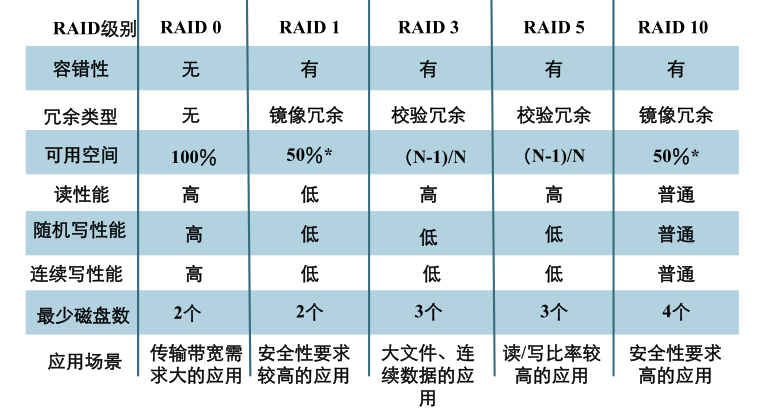
\includegraphics[width=0.8\linewidth]{figures/screenshot008}
	\caption{}
	\label{fig:screenshot008}
\end{figure}

\question{存储网络的三种形态比较}
\begin{figure}[H]
	\centering
	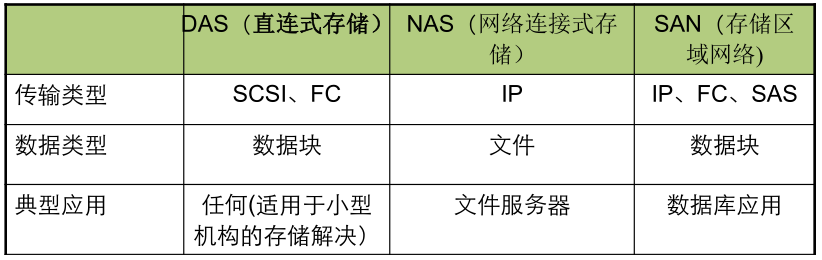
\includegraphics[width=0.8\linewidth]{figures/screenshot009}
	\caption{}
	\label{fig:screenshot009}
\end{figure}


\question{数据库安全}
\begin{description}
	\item[定义] 指保护数据库以防止非法用户访问数据库,造成数据泄露、更改或破坏
	\item[网络环境下] 数据库的安全性与网络系统层、操作系统层、数据库管理系统层有关
\end{description}







